\documentclass[11pt]{article}

\usepackage{graphicx}
\usepackage[rightcaption]{sidecap}

\bibliographystyle{ieeetr}

\title{Generative Adversarial Network Model for the BRCA1 and BRCA2 Genes}

\author{
    Anders Poirel, James Casaletto \\ 
    Computational Genomics Lab \\
    University of Califonia, Santa Cruz
}
\date{Fall 2020}


\begin{document}

\maketitle

\section{Introduction}

Sharing genetic data raises a number of privacy challenges due to the possibility 
of attacks that can re-identify indivuals in the dataset,
whose dissemination is often highly restricted as a protective measure \cite{erlich2014routes, aziz2019privacy} 
On the other hand, these restrictions have an adverse effect on the utility of 
these datasets to future research \cite{erlich2014routes, aziz2019privacy}.
Several works propose the use of generative models to reconcile these conflicting
demands \cite{chen2018differentially, yelmen2019creating}. The hope is that these 
models will enable the dissemination of synthetic samples where the original 
indiviuals will not be re-indentifiable, while preserving enough of the structure
if the original data that it still has research utility. \\

This paper explores potential generative models to enable this application on genotype 
data for the BRCA1 and BRCA2 genes. 

\section{Methods}

\subsection{Data pre-processing}

The source datasets consists the of the genotypes of 10,307 indiduals for the BRCA1 and
BRCA2 genes, stored in VCF format. As the generative model expects inputs of the form 
of a nucleotide sequence for the gene of interest, it is necessary to reconstruct the 
entire sequence from each haplotype. For both copies of the gene for each individual in
 the dataset, a sequence is created by replacing positions in the reference genome with
  the alternative allele if the individual has it. \\

For simplicity, only SNP variants were considered. Accounting for deletions and complex 
substitutions would increase considerably the complexity of this process as it would no 
longer be possible to rely on a stable position index while reconstructing the 
sequence. This choice also simplifies considerably modeling and interpretating results
 as one can assume that all input and ouptut sequences will be of the same length.

This approach nevertheless preserves most of the original data given that 91\% of 
variants in the dataset are SNPs. \\


The pre-processing code uses \texttt{BioPython} \cite{cock2009biopython} for I/O on FASTA files,
and \texttt{scikit-allel} \cite{miles2017scikit} for I/O on VCF files.

\subsection{Model}

\subsubsection{Review of generative models}

Several generative models for anonymizing data and/or creating DNA sequences
have been proposed. These suitability of each is briefly reviewed below. \\ 

\textbf{Variational Autoencoders (VAEs)}

Variants of variational autoencoders are explored in ref. \cite{chen2018differentially} as an approach for anonymizing data, finding that VAEs are effectively able to mitigate
privacy loss without sacrificing data utility. 
Furthermore, VAEs can incorporate a variety of architectural heuristics tuned to the 
structure of the data (e.g. convolutional layers when the data has a known topological 
structure).
However, the authors in ref. \cite{killoran2017generating} found that VAEs performed 
poorly on real world genomic data, ignoring entirely latent codes, and suggested that
 this is a result of the noisyness of genetic data. \\


\textbf{Restricted Boltzmann Machines (RBMs)}

RBMs are in principle suitable for the purposes of generating DNA, but experiments with 
RBMs for this purpose show that while their output can be competitive with other approache,
training is failure-prone \cite{yelmen2019creating}. 
Furthermore, training RBMs is in general difficult. RBMs are trained with 
Markov Chain Monte Carlo \cite{fischer2014training}, which available computational engines cannot accelerate to the same extent as gradient descent based optimization. 
This makes using RBMs on datasets of the (modest) scale considered here unpractical. \\


\textbf{Generative Adversarial Networks (GANs) }

Severals experiments have shown GANs to be an effective approach to generating genetic
data \cite{killoran2017generating, yelmen2019creating}. Using gradient penalty methods, 
Wasserstein GANs can be trained reliably \cite{gulrajani2017improved} and efficiently, 
while reliably leveraging latent codes \cite{killoran2017generating}.

Furthermore, like VAEs, GAN architecture can be tuned to the structure of specific 
types of data. Here, this approach can leverage the fact that genetic data has a 
structure that sits somewhere between that of natural language text and images 
\cite{killoran2017generating} - it is a discrete sequence of characters with 
higher-level structure, and has repeating motifs (for instance, codons) overlaid on 
a ``noisier'' background (for instance, non-coding DNA). Thus, it is desirable for 
the chosen modeling approach to be capable of incorporating heuristics developed for 
both types of data: in ref. \cite{killoran2017generating} the authors use an 
architecture incorporating both 1D convolutions and residual connections. 

\subsubsection{Model Details}

As discussed above, the model proposed in ref. \cite{killoran2017generating} is 
particularly well-suited to the problem at hand, so the architecture here is a direct 
implementation of the one described in that paper. \\

    
\begin{SCfigure}[0.5][h]
    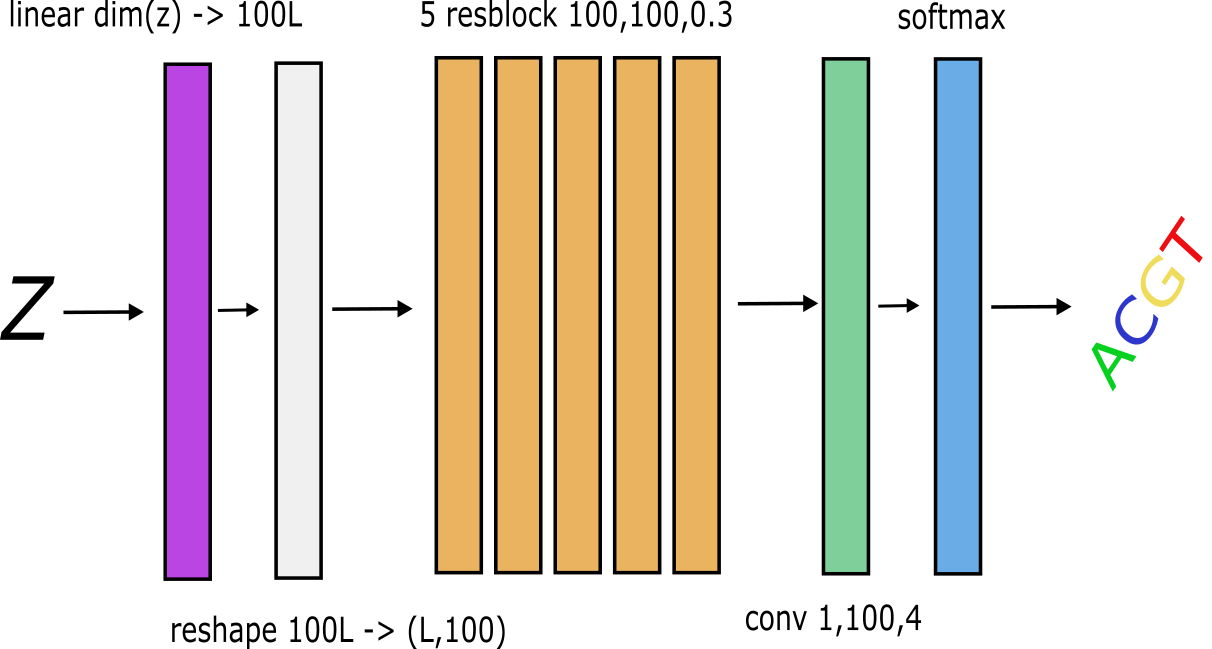
\includegraphics{generator.png}
    \caption{Generator architecture}
\end{SCfigure}

The generator consists of a linear layer which maps the latent code into 
a higher dimensional space, followed by five residual blocks then a convolutional layer which maps the output to a sequence of dimension  $(L, 4)$.

\begin{SCfigure}[0.5][h]
    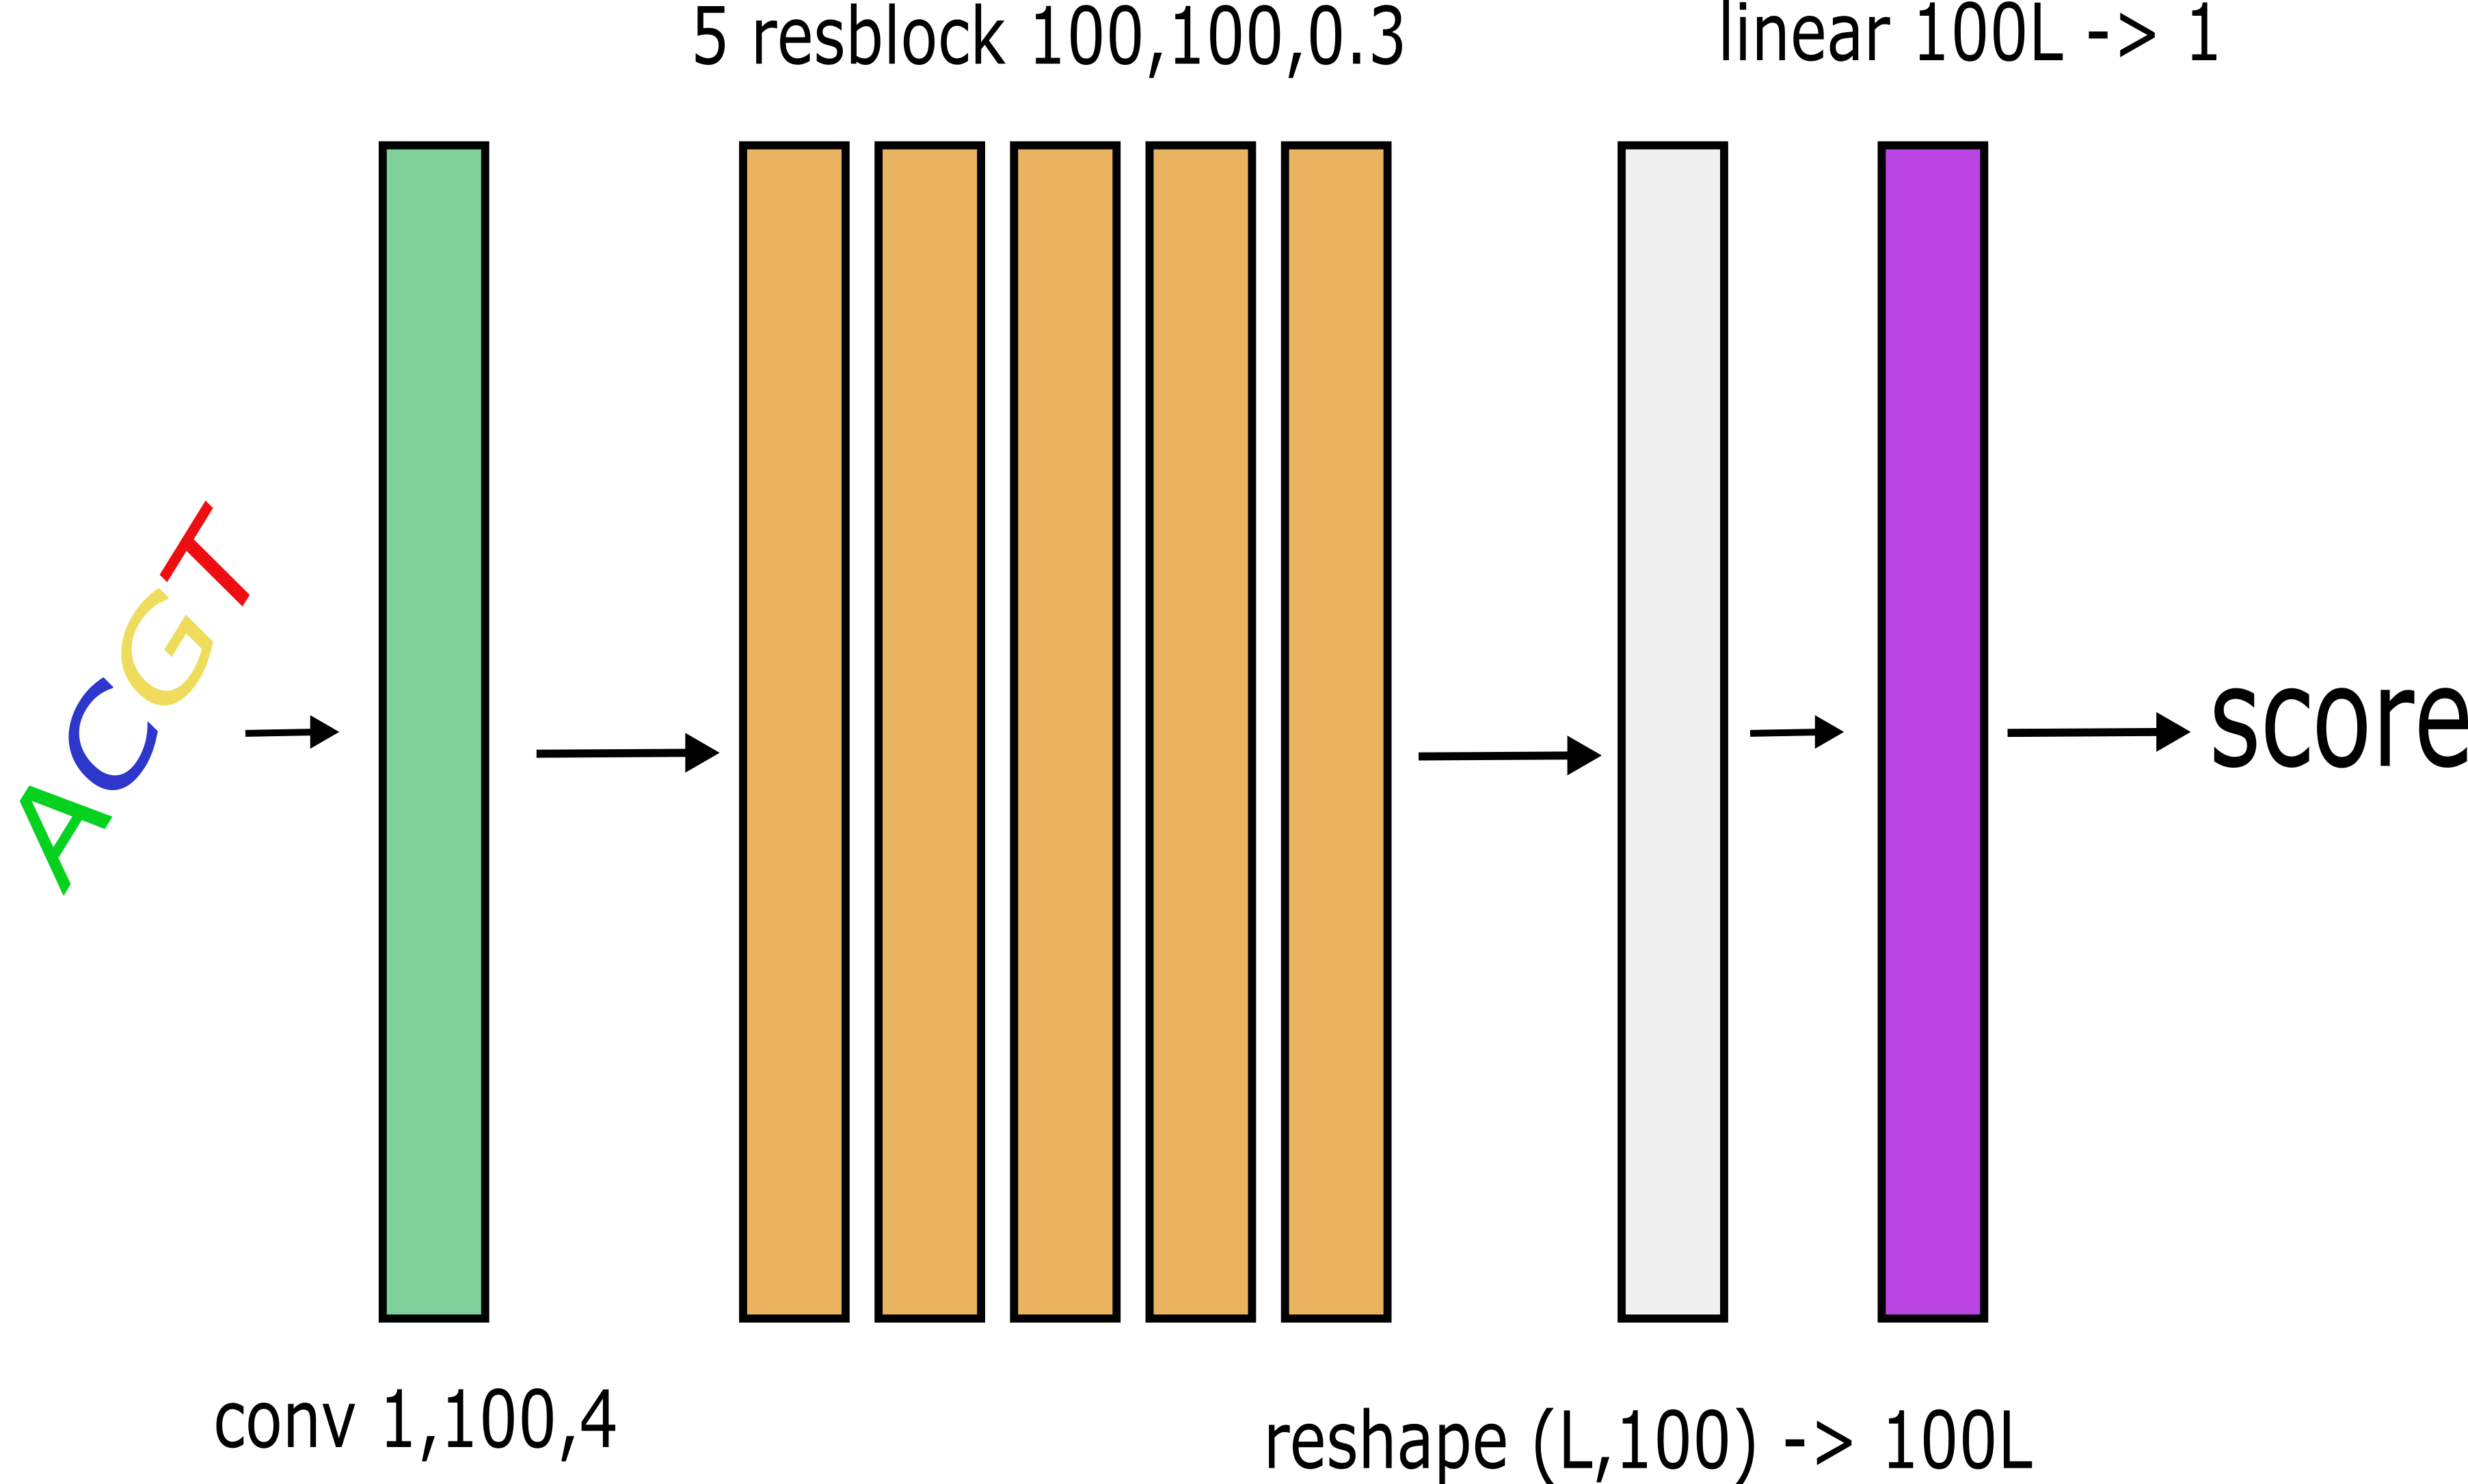
\includegraphics{discriminator.png}
    \caption{Discriminator architecture}
\end{SCfigure}

The discriminator is almost symmetric to the generator, outputting a score 
quantifying the networks' confidence that the input sequence is real.

\begin{SCfigure}[0.5][h]
    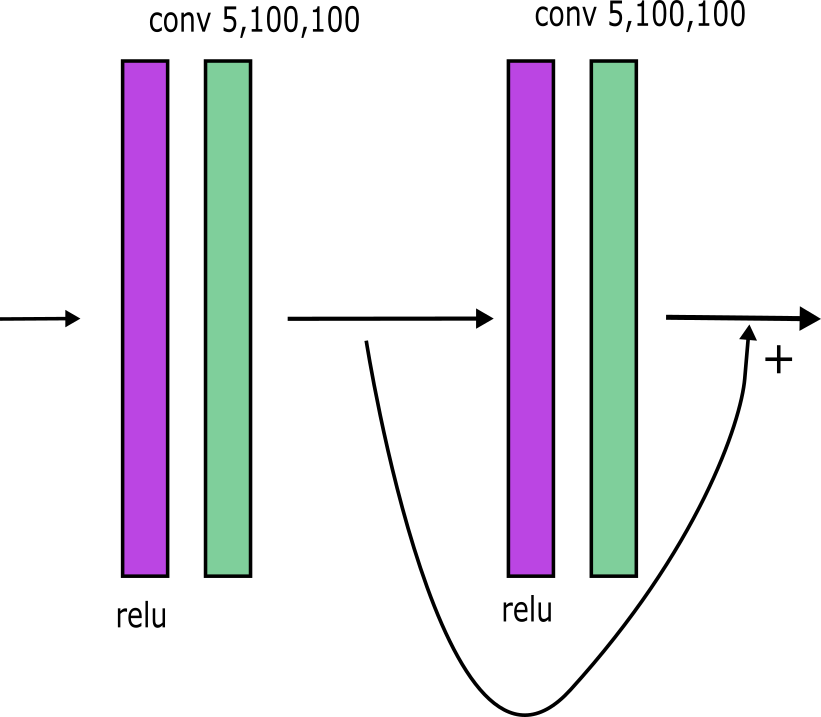
\includegraphics{resblock.png}
    \caption{Residual block architecture}
\end{SCfigure}

The residual blocks consist of stacked 1D convolutional and linear layers, motivated by the heuristic that the 1D convolution parameters will encode reapeating motifs in DNA.

After training, the generator can be used to creating of data by sampling from 
the latent space. \\

The model was implemented in PyTorch 1.7 \cite{paszke2019pytorch}, following the 
original Tensorflow implementation of the architecture described in 
\cite{killoran2017generating}.

\section{Results}


While the residual layers have a constant number of parameters given 
a fixed latent space dimension $D_z$, the cost of the linear first layer in the generator 
and last  layer in the discriminator increases rapidly with the the 
sequence length $L$. FOr instance, the number of learnable parameters associated 
with the fisrst layer of the generator is given by
\[
    (100 D_z \cdot + 100)L   
\] 
The results in \cite{killoran2017generating} used $D_z = 100$. Using the same 
architecture on the full BRCA1 sequence thus requires 1,272,095,000 learnable 
parameters just for the first linear layer. With standard training batch sizes (32 or 64),
the model's memory consumption thus becomes prohibitely large for training on a single
GPU.
% (see Appendix B for a more in-depth exploration).

\subsection{Discussion}

The architecture proposed in \cite{killoran2017generating} was originally tested with 
sequences that were 50 and 500 bases long. The above results show that extending 
this model to longer sequences of tens or hundreds of thousands of bases long is unweildy
due to the number of parameters involved. \\
While no model was trained due to this, the number of parameters suggests other 
potential issues with the approach. While the dataset contains $\sim 10,000$ samples, 
this may not be enough data to reliably train such a large model. \\
Therefore, adapting this approach to longer sequences will likely require a more parsomonious architecture. 

\section{Future work}

There are several possible avenues to reducing the memory consumption of the model.
A successful approach will likely require using a combination of these.
\begin{itemize}
    \item Reducing the latent dimension 
    \item Reducing the dimension of the hidden units (100 in the original version)
    \item Using half-precision datatypes
    \item Distributing the architecture across several GPUs
    \item Modeling sub-sequences of the entire BRCA genes.
\end{itemize}

Once the model is shrunk to a more manageable size, it will be possible to 
evaluate its effectiveness at balancing the tradeoff between privacy and data
quality.


\bibliography{cgl_paper_f20}
    
\newpage

\appendix

\section{Model Notation}

Description of the notation used to describe model layers. This follows 
the notation used in ref. \cite{killoran2017generating}.
\begin{itemize}
    \item \textbf{linear} $y \rightarrow z$: a linear layer with 
    input dimension $y$ and output dimension $z$
    \item \textbf{conv} $x,y,z$: a 1D convolutional layer with kernel 
    size $x$, input dimension $y$ and ouput dimension $z$.
    \item \textbf{resblock} $x,y,z, \alpha$. A residual layer, constituted
    of 2 blocks each with a \textbf{linear} $y \rightarrow z$ layer followed
     by a \textbf{conv} $x,y,z$ layer. The output of the first block is 
    multiplied by $\alpha$ and fed back into the second block.
\end{itemize}

The batch size dimension of each layer is ommitted to simplify notation.

% \section{Exploration of Memory Usage}

% To gain a better understanding of the issues that were encountered, and suggest 
% directions for future work, the model's memory usage was further explored using 
% PyTorch's profiler. The memory consumption of the generator is tested for 
% sequence lengths $L = 50, 500, 5000$, and a batch size of 32. The discriminator's
% linear layer has 100$\times$ fewer parameters than the generator, so the latter 
% will dominate the overall model's memory consumption. 


\end{document}